\documentclass[mathserif,utf8,14pt]{beamer}
\usepackage[utf8]{inputenc}
\usepackage{tikz}
\usepackage[english,russian]{babel}
\usepackage[absolute,overlay]{textpos}
\usepackage{amsmath}
\usepackage{graphicx}

\usetheme{Madrid}
%\setbeamerfont{framesource}{size=\small}
%\setbeamercolor{framesource}{fg=gray}
%\newcommand{\source}[1]{\begin{textblock*}{8cm}(0.5cm,8.7cm)
%    \begin{beamercolorbox}[ht=0.5cm,left]{framesource}
%        \usebeamerfont{framesource}\usebeamercolor[fg]{framesource} source: \itshape{{#1}}
%    \end{beamercolorbox}
%\end{textblock*}}

\makeatletter
\setbeamertemplate{footline}
{
  \leavevmode%
  \hspace{0.92\paperwidth}
  \hbox{%
%  \begin{beamercolorbox}[wd=.333333\paperwidth,ht=2.25ex,dp=1ex,center]{author in head/foot}%
%    \usebeamerfont{author in head/foot}\insertshortauthor%~~\beamer@ifempty{\insertshortinstitute}{}{(\insertshortinstitute)}
%  \end{beamercolorbox}%
%  \begin{beamercolorbox}[wd=.333333\paperwidth,ht=2.25ex,dp=1ex,center]{title in head/foot}%
%    \usebeamerfont{title in head/foot}\insertshorttitle
%  \end{beamercolorbox}%
  \begin{beamercolorbox}[wd=.08\paperwidth,ht=2.25ex,dp=1ex,right]{date in head/foot}%
%    \usebeamerfont{date in head/foot}\insertshortdate{}\hspace*{2em}
    \insertframenumber{} / \inserttotalframenumber\hspace*{2ex} 
  \end{beamercolorbox}}%
  \vskip0pt%
}
\makeatother

\beamertemplatenavigationsymbolsempty

\title{PipInstall: определение проплаченных отзывов}
\author{Михаил Кольцов \\ Борис Симиютин \\ Леся Тищенко \\ Михаил Чернявский}
\vspace*{10px}
\date{\today}
\begin{document}
\begin{frame}
    \maketitle
\end{frame}

\begin{frame}{План рассказа}
    \begin{enumerate}
        \item Описание задачи
        \item Ход работ
            \begin{itemize}
                \item Предметная область
                \item Получение обучающей выборки
                \item Используемые признаки
                \item Используемые методы и библиотеки
            \end{itemize}
        \item Результаты
            \begin{itemize}
                \item Тестирование
                \item Возможности продукта
                \item Видеодемонстрация
            \end{itemize}
    \end{enumerate}
\end{frame}

\begin{frame}{Описание задачи}
    \begin{itemize}
        \item делаем классификатор, он обучается на размеченных данных
        \item определяет хорошие отзывы
        \item и плохие (проплаченные) отзывы
    \end{itemize}
    Решили смотреть только на положитьельные отзывы.
\end{frame}

\begin{frame}{Хороший отзыв}
     \addtocounter{framenumber}{-1}
    Достоинства:оповещение по смс, нет очереди, хорошие продавцы, удобный режим работы

    Недостатки:многого нет в наличии

    Комментарий: советую, спасибо
\end{frame}

\begin{frame}{Плохой отзыв}

     \addtocounter{framenumber}{-1}
                Живу в отдаленном районе, в шаговой доступности есть 
                только продуктовые магазины. 
                Купить телефон удобнее всего с помощью Яндекс.маркета. 
                Я и нашел, 
                где можно подешевле купить нормальный аппарат. 
                Предложение от Opt-Device мне понравилось. 
                Ну я у них и заказал. Позвонил в магазин, уточнил, смогут ли завтра привезти. 
                Менеджер подтвердил, что всё будет так, как я прочитал на сайте. 
                На следующий день приехал курьер и привез мой телефон.
\end{frame}

\begin{frame}{Предметная область}
    Выбирали из четырёх тем:
    \begin{enumerate}
        \item магазины;
        \item стоматологии;
        \item отели;
        \item видео на YouTube.
    \end{enumerate}
    Каждый взял по одной теме и искал отзывы. После 1.5 часов посовещались
    и выбрали \textbf{магазины}.
\end{frame}

\begin{frame}{Обучающая выборка}
    Выделили <<маркеры>> для проплаченных отзывов:
    \begin{enumerate}
        \item мало конкретики;
        \item длинная предыстория;
        \item смайлики и восклицательные знаки;
        \item чем длиннее отзыв, тем более подозрительный;
        \item мало ошибок или очень глупые ошибки.
    \end{enumerate}
    Это не идеальная формула -- в зависимости от настроения и человека 
    восприятие отзыва может
    меняться. \\
\end{frame}

\begin{frame}{Обучающая выборка}
     \addtocounter{framenumber}{-1}
    Кроме того, задавали вопросы профессиональным составителям отзывов:
    \begin{enumerate}
        \item длинный отзыв -- скорее всего липовый;
        \item утрированная эмоциональность от женского лица, безэмоциональность
            от мужского;
        \item все магазины покупают отзывы. 
    \end{enumerate}
\end{frame}

\begin{frame}{Обучающая выборка}
     \addtocounter{framenumber}{-1}
    Магазин \textit{подозрительный}, если у него мало отзывов и более 
    90\% из них положительные.
    \begin{columns}
        \column{0.30\textwidth}
        \begin{itemize}
            \item МВидео 
            \item МТС 
            \item Мегафон 
            \item Эльдорадо 
        \end{itemize}
        \column{0.33\textwidth}
        \begin{itemize}
            \item Landcom 
            \item Opt-Device  
            \item Telebar.ru 
            \item SLK-Service.ru 
            \item BONCH.PRO 
            \item ProAnima.RU 
        \end{itemize}
        \column{0.33\textwidth}
        \begin{itemize}
            \item Cifrovoi.com
            \item Apple-Zone
        \end{itemize}
    \end{columns}
\end{frame}

\begin{frame}{Обучающая выборка}
     \addtocounter{framenumber}{-1}
     \begin{itemize}
         \item собираем по 100 отзывов для каждого магазина;
         \item всего 1200 отзывов;
         \item используем API Я.Маркета, всё храним в JSON;
         \item размечаем в самописном интерфейсе.
     \end{itemize}
\end{frame}

\begin{frame}{Обучающая выборка}
\begin{itemize}
         \item размечаем в самописном интерфейсе.
         \item вот в таком:
     \end{itemize}
     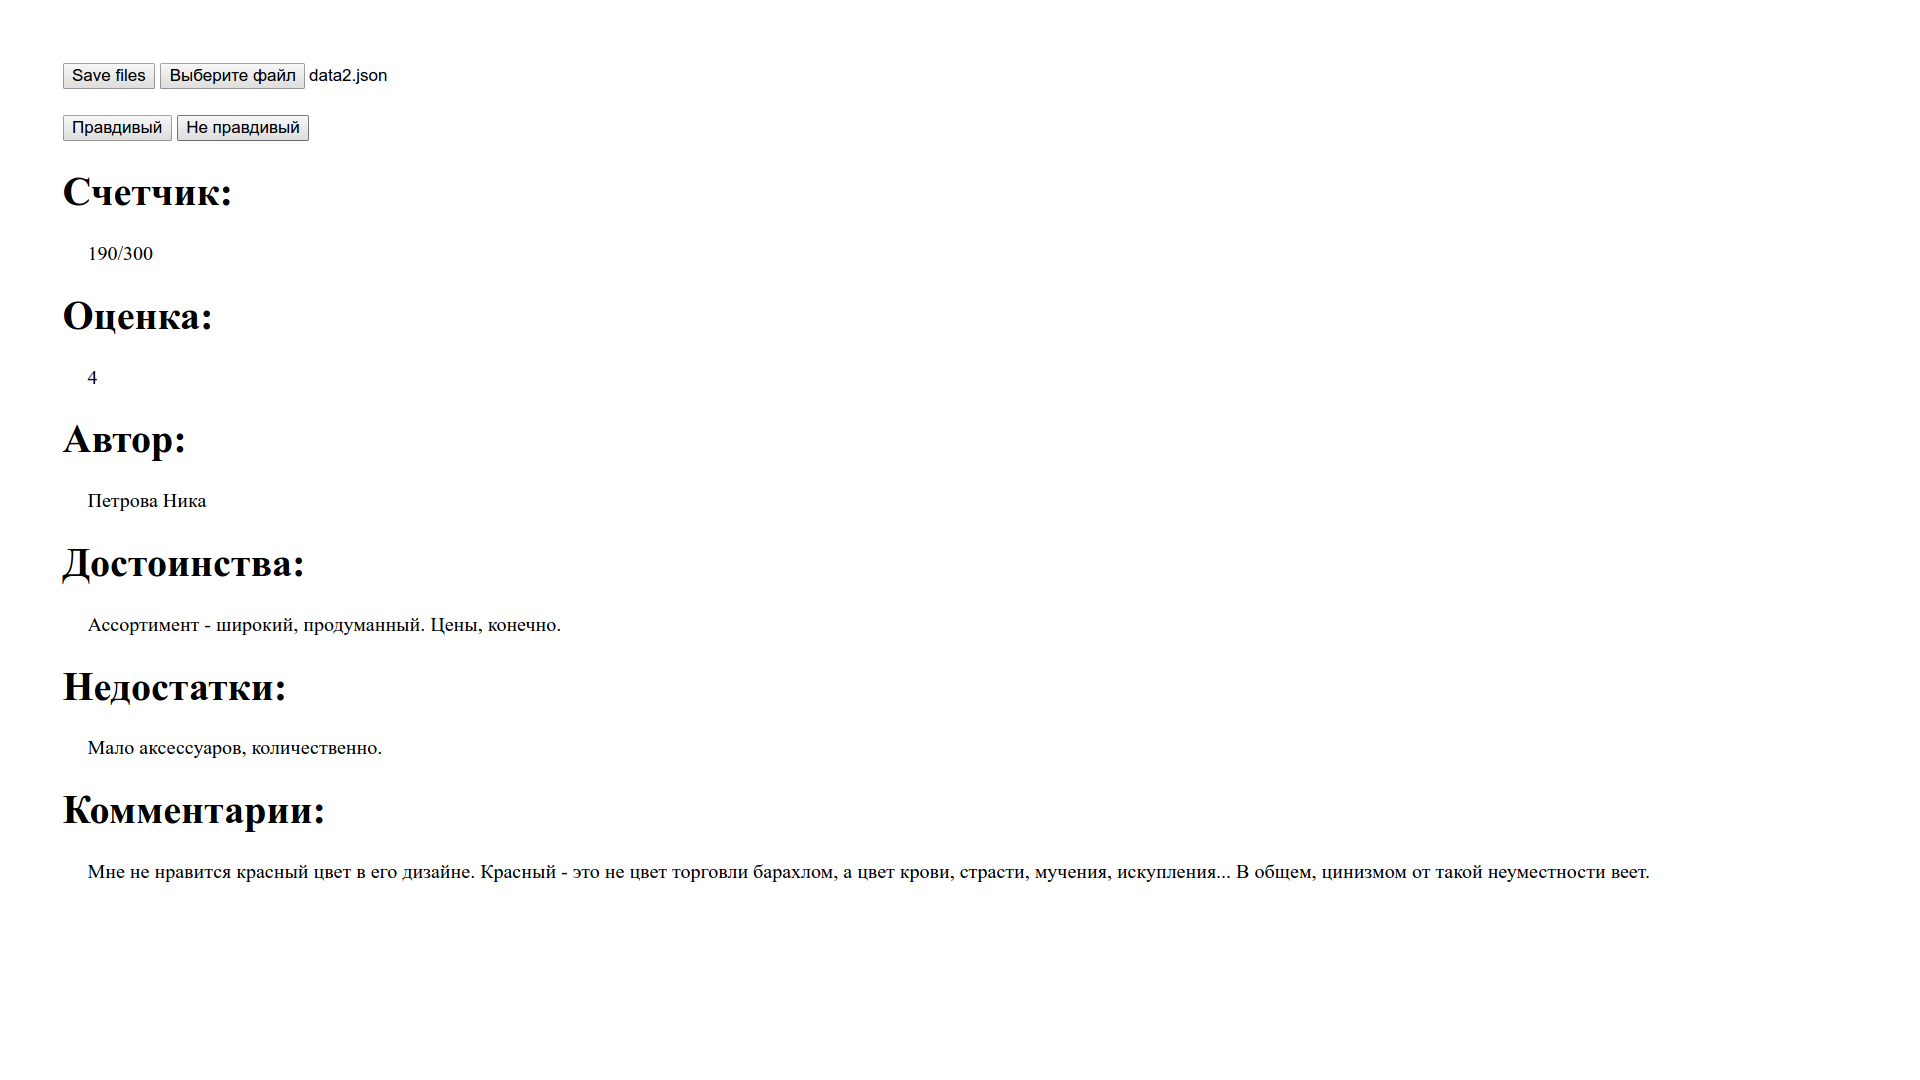
\includegraphics[width=\linewidth]{labeling_interface.png}
\end{frame}

\begin{frame}{Обучающая выборка}
     \begin{itemize}
	 \item каждый голосует за каждый отзыв, считает ли он его проплаченным или нет
         \item результаты разметки:
	 \begin{itemize}	
              \item двое и более проголосовало за один вариант: 714 хороших, 300 проплаченных
              \item решение единогласное: 255 хороших, 42 проплаченных
 	 \end{itemize}
	 \item единогласных маловато
     \end{itemize}
\end{frame}

\begin{frame}{Используемые признаки}
    \begin{itemize}
        \item количество местоимений в первом/втором лице;
        \item количество КАПСОВЫХ слов;
        \item длина отзыва;
        \item количество противопоставлений;
        \item гистограмма частей речи;
    \end{itemize}
\end{frame}

\begin{frame}{Используемые признаки}
     \addtocounter{framenumber}{-1}
    \begin{itemize}
        \item гистограмма букв/слов в отзыве;
        \item количество смайликов, восклицательных знаков;
        \item средняя длина слова;
        \item количество синонимов внутри отзыва;
        \item мета-информация: об авторе, о магазине, $\ldots$
        \item количество грамматических ошибок.
    \end{itemize}
    Ссылки на реализацию: \url{https://github.com/ItsLastDay/PipInstall/wiki/ML-features}
\end{frame}

\begin{frame}{Анализ полезности признаков}
    Здесь слайд(ы) про то, какие признаки как повлияли на качество классификатора;
    как мы оценивали полезность (в том числе визуально) и т.п.
\end{frame}

\begin{frame}{Используемые методы и библиотеки}
    \begin{itemize}
        \item библиотеки: enchant, nltk, pymystem3, sklearn, matplotlib;
        \item нашли словарь синонимов;
        \item поизучали литературу по review spam detection, особенно
            <<Crawford M. et al. Survey of review spam detection using machine learning techniques //Journal of Big Data. – 2015.>>;
        \item реализовали метод по расширению размеченных данных.
    \end{itemize}
\end{frame}

\begin{frame}{Используемые методы и библиотеки}
    Здесь слайд(ы) про то, как мы использовали какие библиотеки,
    какие классификаторы пробовали, как выбирали.
\end{frame}

\begin{frame}{Результаты. Тестирование}
    \begin{itemize}
        \item взяли отзывы, по которым есть консенсус среди размечавших;
        \item отложили часть из них для тестирования;
        \item расширили данные с помощью неразмеченных отзывов;
        \item обучились, протестировались.
    \end{itemize}
\end{frame}

\begin{frame}{Результаты. Тестирование}
     \addtocounter{framenumber}{-1}
     \begin{center}
        \Huge ~65\%
     \end{center}
\end{frame}

\begin{frame}{Результаты. Сравнение}
     \addtocounter{framenumber}{-1}
     \begin{columns}
         \column{\dimexpr\paperwidth-10pt}
     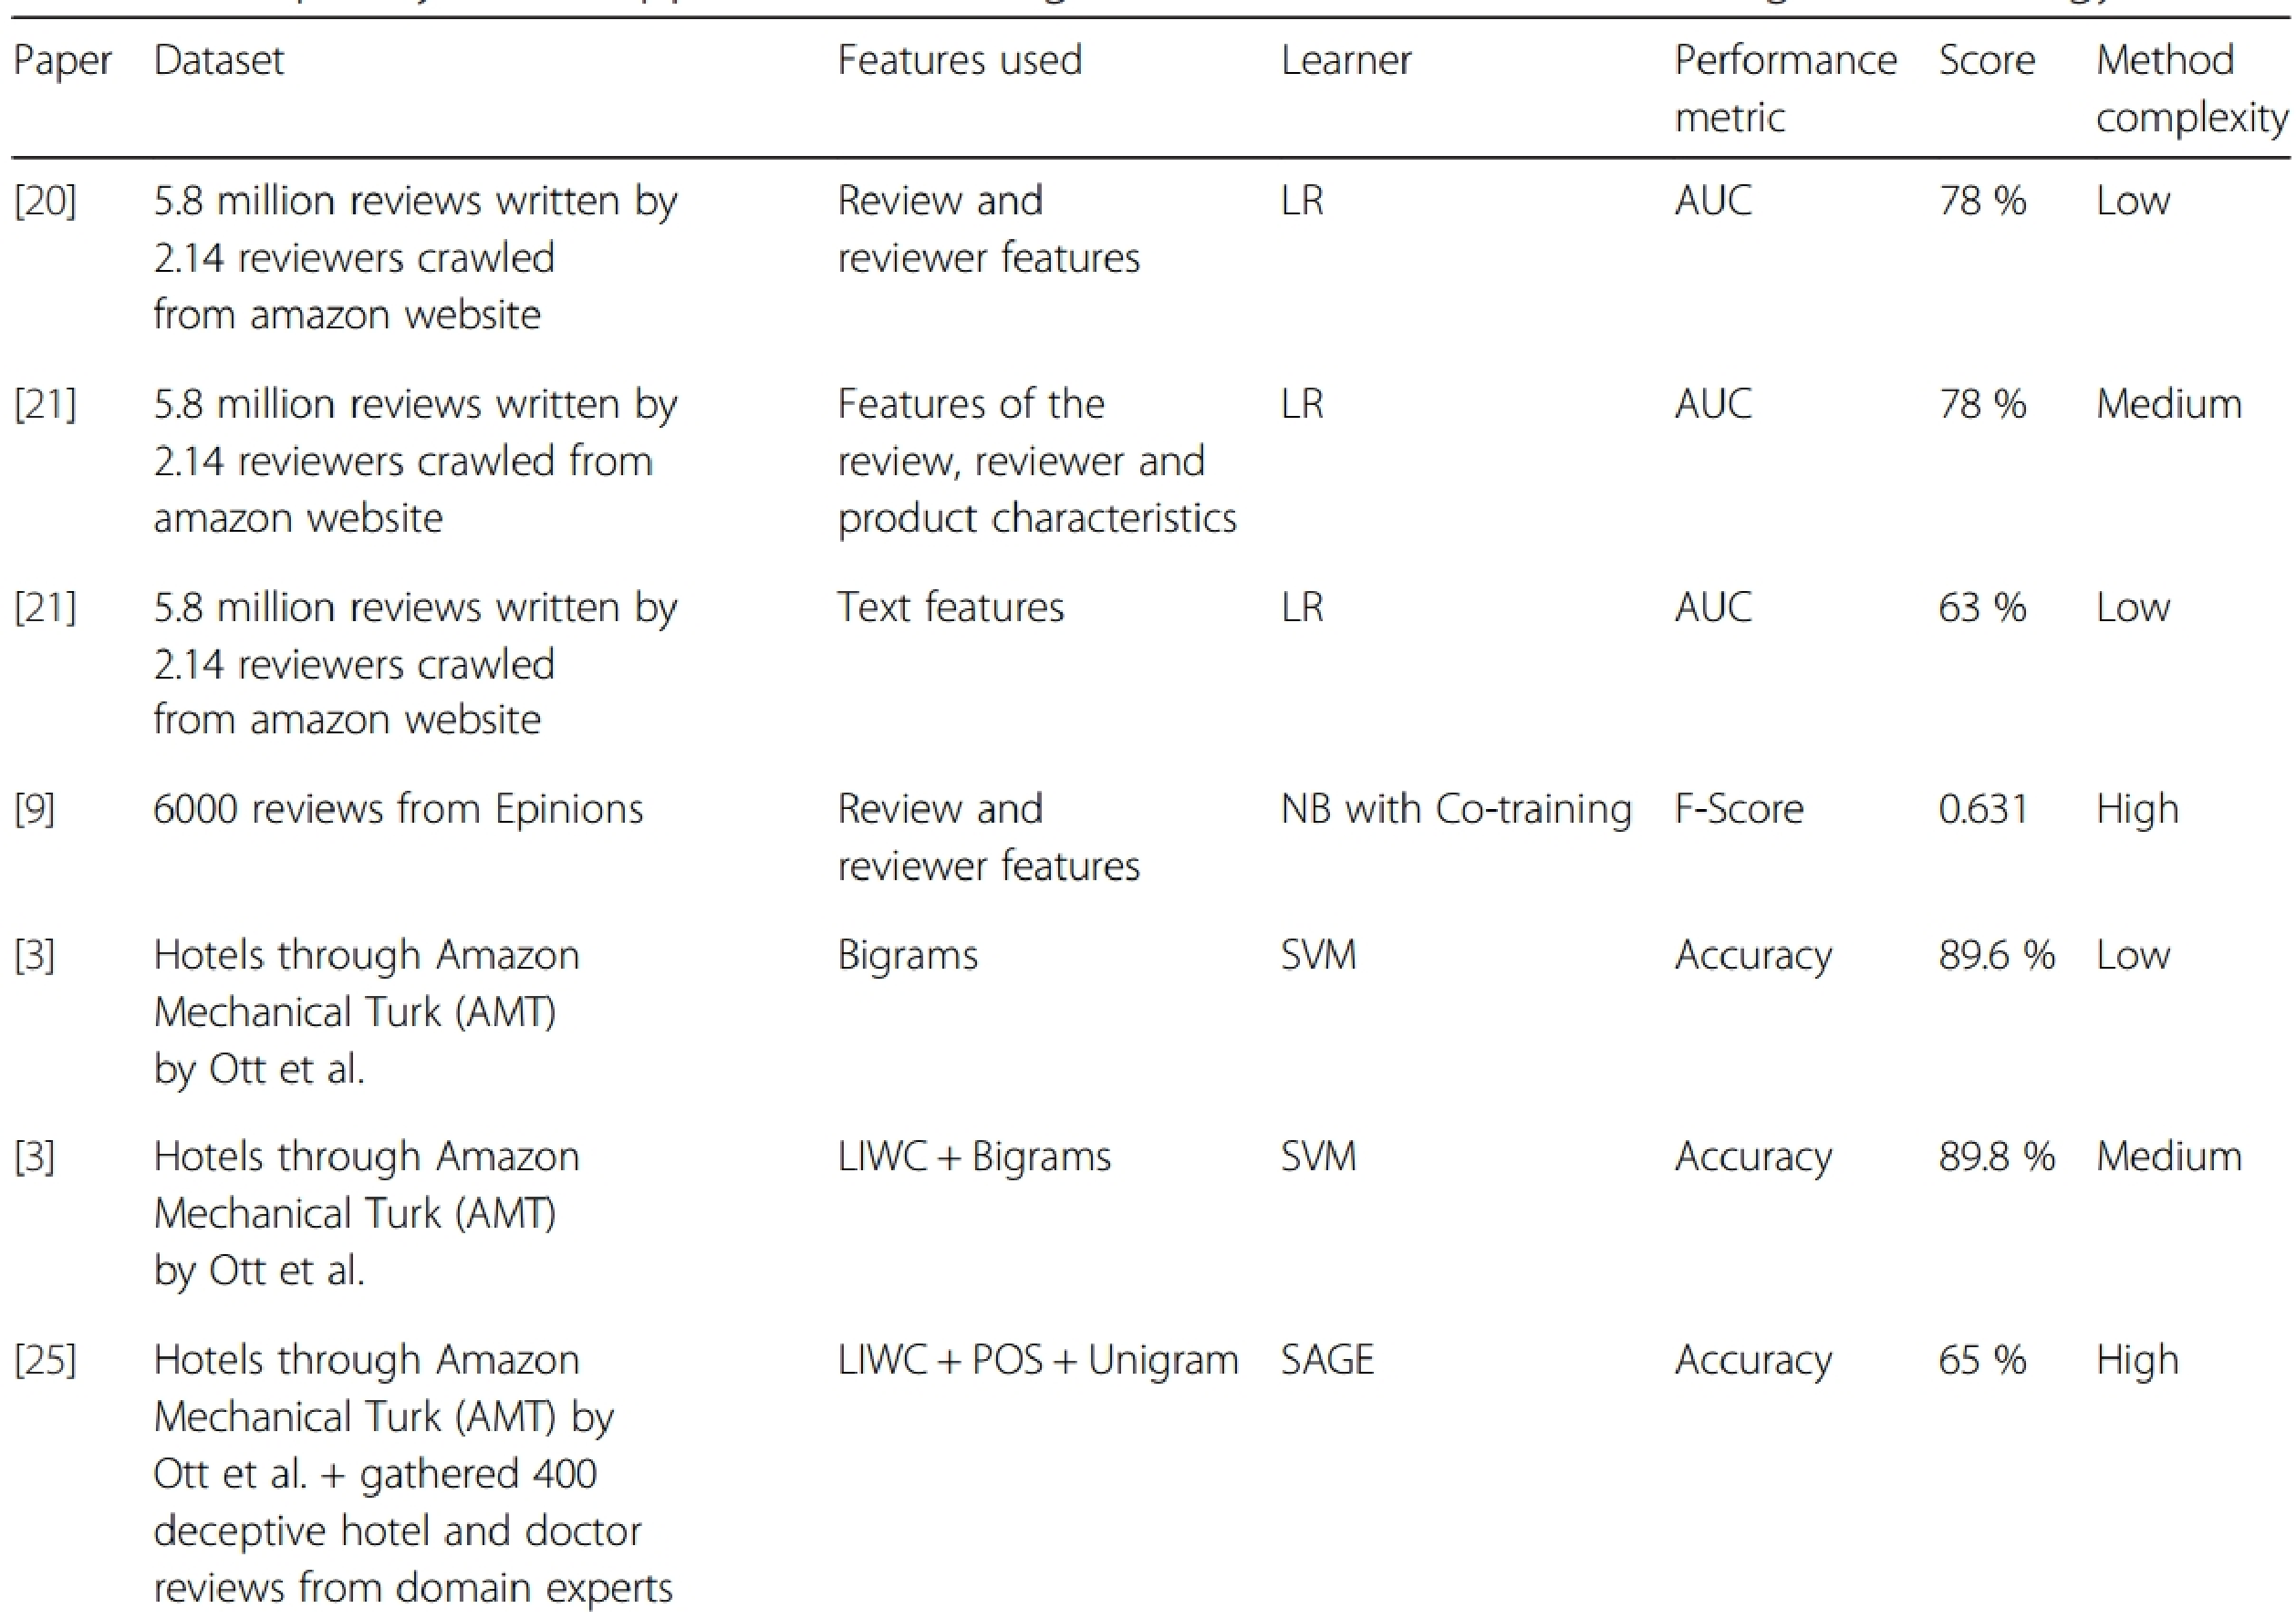
\includegraphics[scale=0.3]{./converted_jpg.pdf}
     \end{columns}
\end{frame}

\begin{frame}{Возможности продукта}
    \begin{itemize}
        \item натравливаем классификатор на отзывы с Я.Маркета => он даёт ответы;
        \item работает быстро;
        \item результат работы спорный.
    \end{itemize}
\end{frame}

\begin{frame}{Видеодемонстрация}
    \begin{center}
        \url{https://youtu.be/1cF34TQc-vQ}
    \end{center}
\end{frame}
 
\begin{frame}{}
     \addtocounter{framenumber}{-1}
    \begin{center}
    \large Спасибо за внимание!
    \end{center}
\end{frame}

\end{document}
